\documentclass[12pt,a4paper]{article}
\usepackage{ctex}
\usepackage{amsmath,amscd,amsbsy,amssymb,latexsym,url,bm,amsthm}
\usepackage{epsfig,graphicx,subfigure}
\usepackage{enumitem,balance}
\usepackage{wrapfig}
\usepackage{mathrsfs,euscript}
\usepackage[usenames]{xcolor}
\usepackage{hyperref}
\usepackage[vlined,ruled,linesnumbered]{algorithm2e}
\usepackage{array}
\hypersetup{colorlinks=true,linkcolor=black}

\newtheorem{theorem}{Theorem}
\newtheorem{lemma}[theorem]{Lemma}
\newtheorem{proposition}[theorem]{Proposition}
\newtheorem{corollary}[theorem]{Corollary}
\newtheorem{exercise}{Exercise}
\newtheorem*{solution}{Solution}
\newtheorem{definition}{Definition}
\theoremstyle{definition}

\renewcommand{\thefootnote}{\fnsymbol{footnote}}

\newcommand{\postscript}[2]
 {\setlength{\epsfxsize}{#2\hsize}
  \centerline{\epsfbox{#1}}}

\renewcommand{\baselinestretch}{1.0}

\setlength{\oddsidemargin}{-0.365in}
\setlength{\evensidemargin}{-0.365in}
\setlength{\topmargin}{-0.3in}
\setlength{\headheight}{0in}
\setlength{\headsep}{0in}
\setlength{\textheight}{10.1in}
\setlength{\textwidth}{7in}
\makeatletter \renewenvironment{proof}[1][Proof] {\par\pushQED{\qed}\normalfont\topsep6\p@\@plus6\p@\relax\trivlist\item[\hskip\labelsep\bfseries#1\@addpunct{.}]\ignorespaces}{\popQED\endtrivlist\@endpefalse} \makeatother
\makeatletter
\renewenvironment{solution}[1][Solution] {\par\pushQED{\qed}\normalfont\topsep6\p@\@plus6\p@\relax\trivlist\item[\hskip\labelsep\bfseries#1\@addpunct{.}]\ignorespaces}{\popQED\endtrivlist\@endpefalse} \makeatother

\begin{document}
\noindent

%========================================================================
\noindent\framebox[\linewidth]{\shortstack[c]{
\Large{\textbf{Lab09-Network Flow}}\vspace{1mm}\\
CS214-Algorithm and Complexity, Xiaofeng Gao \& Lei Wang, Spring 2021.}}
\begin{center}
\footnotesize{\color{blue}$*$ Name:\underline{\quad   Haoyi You  \quad  }\quad Student ID:\underline{\quad 519030910193 \quad} \quad Email: \underline{\quad yuri-you@sjtu.edu.cn \quad}}
\end{center}

\begin{enumerate}
    \item  Consider there is a network consists $n$ computers. For some pairs of computers, a wire $i$ exists in the pair, which means these two computers can communicate with each other. When a signal passes through the wires, the noise in the signal will be amplified.If you know the magnification rate of noise $m_{i,j}$ of each wire (which must be greater than 1). Design an algorithm to find the route  for each other computer to send signals to the computer $v$ with the minimum total magnification rate of noise and analyze the time complexity.
    \begin{solution}
    We define $n_{i,j}=ln(m_{i,j})$, thus if the route from $u$ to $v$ has the minimum noise $m=\prod \limits_{e\in path}m_e$, the $ln(m)=\sum \limits_{e\in path}n_e$ is also the minimum,thus we can change the problem to finding the shortest path problem, then we apply the Dijkstra algorithm.\\
    	\begin{algorithm}[H]
		\KwIn{$G(V,E,M)$, a specific vertex $v_0$}
		\KwOut{Minimum noise $M$ of $V$}
		
		\BlankLine
		\caption{minimum noise}\label{noise}
		set $V'$\\
		\For{$v \in V$}{
		    \If{$e=(v,v_0)\in E$}{$d_{v,v_0}\leftarrow ln(m_{v,v_0})$}
		    \Else{$d_{i,j}\leftarrow \infty$}
		    $V'.insert(v)$
		}
		\While{$V'$ is not empty}{find $v'\in V'$ with $d_{v_0,v'}$ is minimal\\
		    $V'.pop(v')$\\
            \For{$v\in V'$}{
 		    $d_{v_0,v}\leftarrow min(d_{v_0,v'}+ln(m_{v,v'}),d_{v_0,v})$
 		    }
		}
		\For{$v \in V$}{
		    $M_v\leftarrow exp(d_{v_0,v})$
		}
		\Return M
	\end{algorithm}
	Time complexity: in while loop it recursive $|V|$ times, and in each recursion the for loop it cost $|V'|$.So the complexity is $\sum \limits_{i=1}^{|V|}|V|-i=O(|V|^2)$.\\
	Space complexity: storing the edges and noise needs $O(|E|)$ space, and storing $d,V',M$ cost $O(|V|)$ space, so the total complexity is $O(|E|+|V|)$
    \end{solution}
	
	\item Suppose that we wish to maintain the transitive closure of a directed graph $G=(V,E)$ as we insert edges into $E$. That is, after each edge has been inserted, we want to update the transitive closure of the edges inserted so far. Assume that the graph $G$ has no edges initially and that we represent the transitive closure as a boolean matrix.
	\begin{enumerate}
	    \item Show how to update the transitive closure of a graph $G=(V,E)$ in $O(V^2)$ time when a new edge is added to $G$.
	    \item Give an example of a graph $G$ and an edge $e$ such that $\Omega(V^2)$ time is required to update the transitive closure after the insertion of $e$ into $G$, no matter what algorithm is used.
	    \item Describe an efficient algorithm for updating the transitive closure as edges are inserted into the graph. For any sequence of $m$ insertions, your algorithm should run in total time $\sum_{i=1}^m t_i=O(V^3)$, where $t_i$ is the time to update the transitive closure upon inserting the $i$th edge. Prove that your algorithm attains this time bound.
	\end{enumerate}
	\begin{solution}
	\begin{enumerate}
	    \item 
	~\par
	 \begin{algorithm}[H]
	 \KwIn{graph $G=(V,E)$,boolen matrix $M$,an edge $e=(v_i,v_j)$}
	\KwOut{Modified $M$}
    \caption{update once transitive closure}\label{transitive}
    \For{$v_1\in V$}{
        \For{$v_2\in V$}{
            $M_{v_1,v_2}\leftarrow M_{v_1,v_2}|(M_{v_1,v_i}\& M_{v_j,v_2})$
        }
    }
	\end{algorithm}
	\item
	In the situation that the whole graph is dichotomous complete graph with two parts $G_1,G_2$, each part has $\frac{|V|}{2} vertexs$, choose $v_1\in G_1,v_2\in G_2$,add $(v_1,v_2)$ into the graph, and $\forall v_i\in G_1,v_j\in G_2,M_{v_i,v_j}$ change to true from false, so we at least needs to modify $\frac{n^2}{4}=\Omega(n^2)$ datas.
	\item
	\par The algorithm is below.\\
		\begin{algorithm}[H]
	 \KwIn{graph $G=(V,E)$,boolen matrix $M$,a sequence of edges $\{e_i\}=\{(u_i,v_i)\}$}
	\KwOut{Modified $M$}
    \caption{Online updating transitive closure}\label{transitive1}
    \For{$u\in V,v\in V$}{
        \If{$u==v$}{$M_{u,v}\leftarrow$true\\}
        \Else{$M_{u,v}\leftarrow$false\\}
    }
    $\backslash\backslash$ initialization\\
    \For{$e\in \{e_i\}$}{
        $\backslash\backslash$ first layer of loop\\
        \For{$w\in V$}{
        $\backslash\backslash$ second layer of loop\\
            \If{$M_{w,u_i}==true\&M_{w,v_i}==false$}{
               \For{$x\in V$}{
                    $\backslash\backslash$ third layer of loop\\
                    $M_{w,x}\leftarrow M_{w,x}|M_{v_i,x}$
                } 
            }
        }
        $\backslash\backslash$ This time the M is the result after adding $e_i$ 
    }
	\end{algorithm}
	Here we prove the time complexity of this algorithm is $O(n^3)$.\\
	Let $\Phi(i)$ be defined as the number of false elements in boolen matrix M.Obviously, $\Phi(i)=n^2-n=O(n^2)$.\\
	In the algorithm, every time entering into the third layer of loop means $M_{w,v_i}==false$, so if $\Phi(i)==0$, it will never enter into this loop. Assume $t$ is the total time entering into this loop. The complexity of this algorithm is $O(n*t)$\\
	Each time it enters into the loop, $M_{w,v_i}$ will change to true from false, so at least $\Phi(i)$ will minus 1,thus $t\le\Phi(i)=O(n^2)$.\\
	So the total time of complexity is $O(n*t)=O(n^3)$.
	\end{enumerate}
	\end{solution}
	\item An $n\times n$ grid is an undirected graph consisting of n rows and n columns of vertices, as shown in Figure 26.11. We denote the vertex in the $i$th row and the $j$th column by $(i,j)$. All vertices in a grid have exactly four neighbors, except for the boundary vertices, which are the points $(i,j)$ for which $i = 1, i = n, j = 1$, or $j = n$.
    Given $m\leqslant n^2$ starting points $(x_1,y_1), (x_2, y_2), ... , (x_m, y_m)$ in the grid, the escape problem is to determine whether or not there are $m$ vertex-disjoint paths from the starting points to any $m$ different points on the boundary such that every vertex in $V$ is included in at most one of the $m$ paths. For example, the grid in Figure \ref{Fig-EscapeProblem}(a) has an escape, but the grid in \ref{Fig-EscapeProblem}(b) does not.
    \begin{figure}[!htbp]
	\centering
	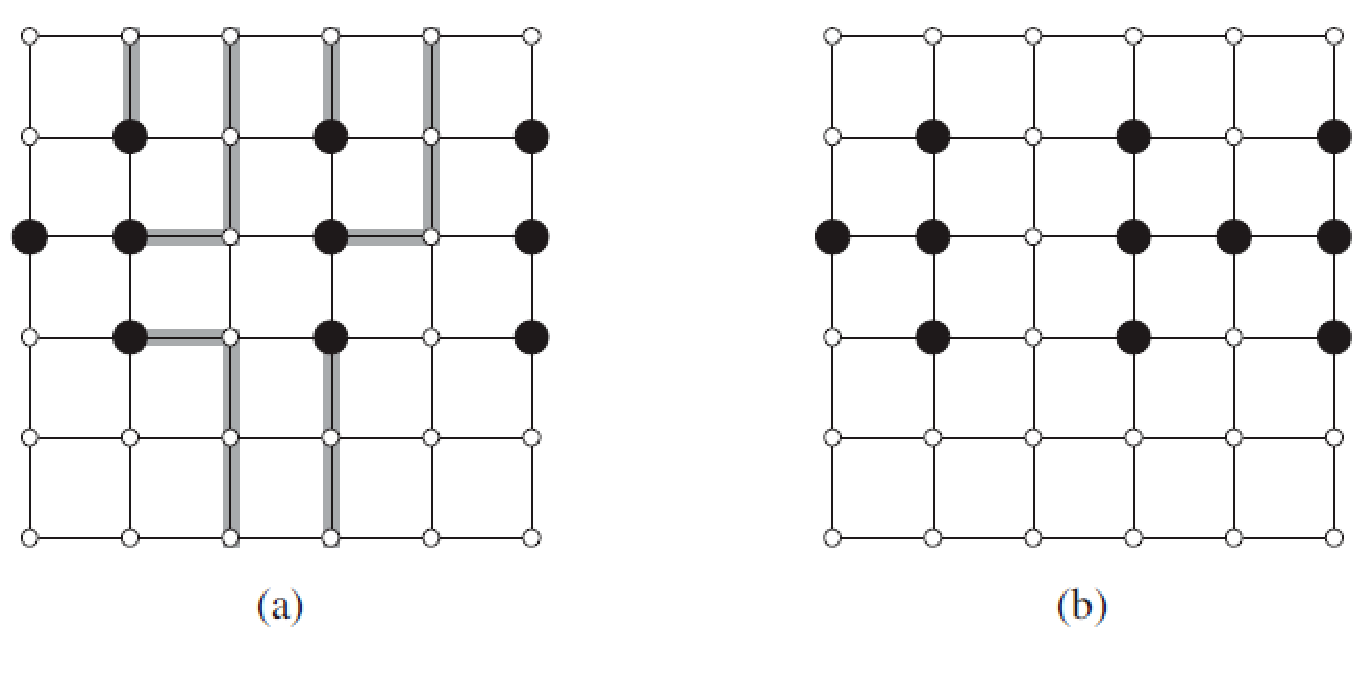
\includegraphics[width=0.5\textwidth]{Fig-EscapeProblem.pdf}
	\caption{Grids for the escape problem. Starting points are black, and other grid vertices are white. (a) A grid with an escape, shown by shaded paths. (b) A grid with no escape.}
	\label{Fig-EscapeProblem}
	\end{figure}
    \begin{enumerate}
        \item Consider a flow network in which vertices, as well as edges, have capacities. That is, the total positive flow entering any given vertex is subject to a capacity constraint. Show that determining the maximum flow in a network with edge and vertex capacities can be reduced to an ordinary maximum-flow problem on a flow network of comparable size. That is, the sizes of the two graph are in the same order of magnitude.
        \item Describe an efficient algorithm to solve the escape problem, and analyze its running time.
    \end{enumerate}
    \begin{solution}
    \item 
    Assume the graph $G=(V,E,M,N)$ with M is the capacity of V and N is the capacity of E.\\
    Firstly,we split each point $v$ into 2 points $v_{in},v_{out}$ that if a directed edge ends at $v$, we change it to end at $v_{in}$. Similarly, if a edge starts from $v$, we change it to start from $v{out}$. The capacity of the edge do not change.\\
    Secondly,for each two splited points $v_{in},v{out}$,we add an edge starting from $v_{in}$ to $v_{out}$ with the capacity of the node $v$.\\
    Thus, the new graph $G'$ has $2|V|$ nodes and $|V|+|E|$ edges, each edge has a capacity from $M$ or $N$, so the sizes of two graph are in the same order of magnitude.
    \item
    The algorithm is below,similar to the algorithm above,change the problem to network flow:\\
    \begin{algorithm}[H]
	 \KwIn{Size $N$,starting points array $A$=\{$(x,y)$\}}
	\KwOut{boolen $Bool$ }
    \caption{Escape}\label{flow}
    % for(
    % \For{$i=1$ \KwTo $N$}{
    %  \For{$j=1$ \KwTo $N$}{
    %     \If{$i==1|i==n|j==1|j==n$}{
    %         $Boundary.insert((i,j))$
    %     }
    %  }
    % }
    % $s\_number\leftarrow sizeof(A)$\\
    % $b\_number\leftarrow sizeof(Boundary)$\\
    % boolen matrix $G[N^2-s\_number-b\_number+1][N^2-s\_number-b\_number+1]\leftarrow 0$
    vertex $source,sink$\\
    $V.insert(source)$\\
    $V.insert(sink)$\\
    \For{$v\in E$}{
        \If{$v\in A$}{
        \For{$u\in V$ and $(v,u)\in E$}{
            $E.delete((v,u))$\\
            $E.insert(source,u)$\\
        }
        $V.pop(v)$
        }
        \Else{
        \If{$v$ in boundary}{
        \For{$u\in V$ and $(u,v)\in E$}{
            $E.delete((u,v))$\\
            $E.insert(u,sink)$\\
        }
        $V.pop(v)$
        }
        \Else{
        vertex $v_in,v_out$
        $V.insert(v_{in})$\\
        $V.insert(v_{out})$\\
        \For{$u\in V$ and $(u,v)\in E$}{
            $E.delete((u,v))$\\
            $E.insert(u,v_{in})$\\
        }
        \For{$u\in V$ and $(v,u)\in E$}{
            $E.delete((v,u))$\\
            $E.insert(v_{out},u)$\\
        }
        $E.insert(v_{in},v_{out}$
        $V.delete(v)$
        }
        }
    }
    initialize $G$ with all edge capacity be 1\\
    $max\leftarrow$ Max-flow(G)\\
    \If{$max==sizeof(A)$}{\Return True}
    \Else{\Return False}
	\end{algorithm}
    Change the graph the same to (a). And merge all the starting points into source and merge all the boundary points(except starting points) into sink. Then the graph has only one sink and source, thus it can apply the Max-flow algorithm mentioned in the class.\\
    Since the merge time complexity is $O(N^4)$ and the max-flow complexity is $O(|V||E|C)$ with $C==1$,$|V|=O(N^2),|E|=O(N^2)$ so the complexity is $O(n^4)$.
    \end{solution}
    
\end{enumerate}

\textbf{Remark:} Please include your .pdf, .tex files for uploading with standard file names.
\newpage


%========================================================================
\end{document}